\section{Bootstrap Your Own Latent (BYOL)}
\begin{frame}{}
    \LARGE Contrastive Learning: \textbf{Bootstrap Your Own Latent (BYOL)}
\end{frame}


\begin{frame}[allowframebreaks]{BYOL (Bootstrap Your Own Latent)}
\begin{figure}
    \centering
    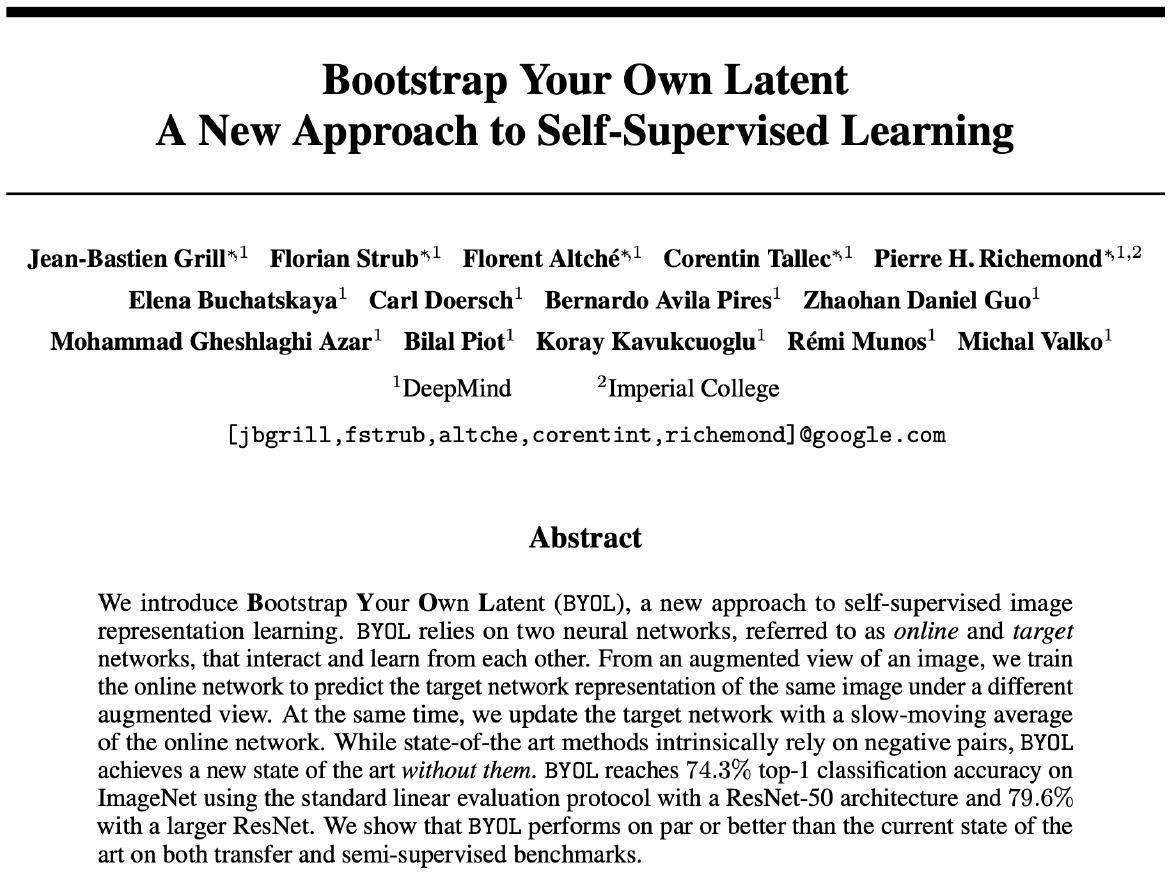
\includegraphics[width=\linewidth,height=0.9\textheight,keepaspectratio]{images/contrastive/slide_80_1_img.jpg}
\end{figure}

\framebreak

\textbf{Why BYOL?}
\begin{itemize}
    \item Most contrastive methods use both positive and negative pairs.
    \item BYOL asks: Can we learn good features without negative pairs?
    \item BYOL shows it is possible to skip negatives and still learn useful representations.
\end{itemize}

\framebreak

\begin{figure}
    \centering
    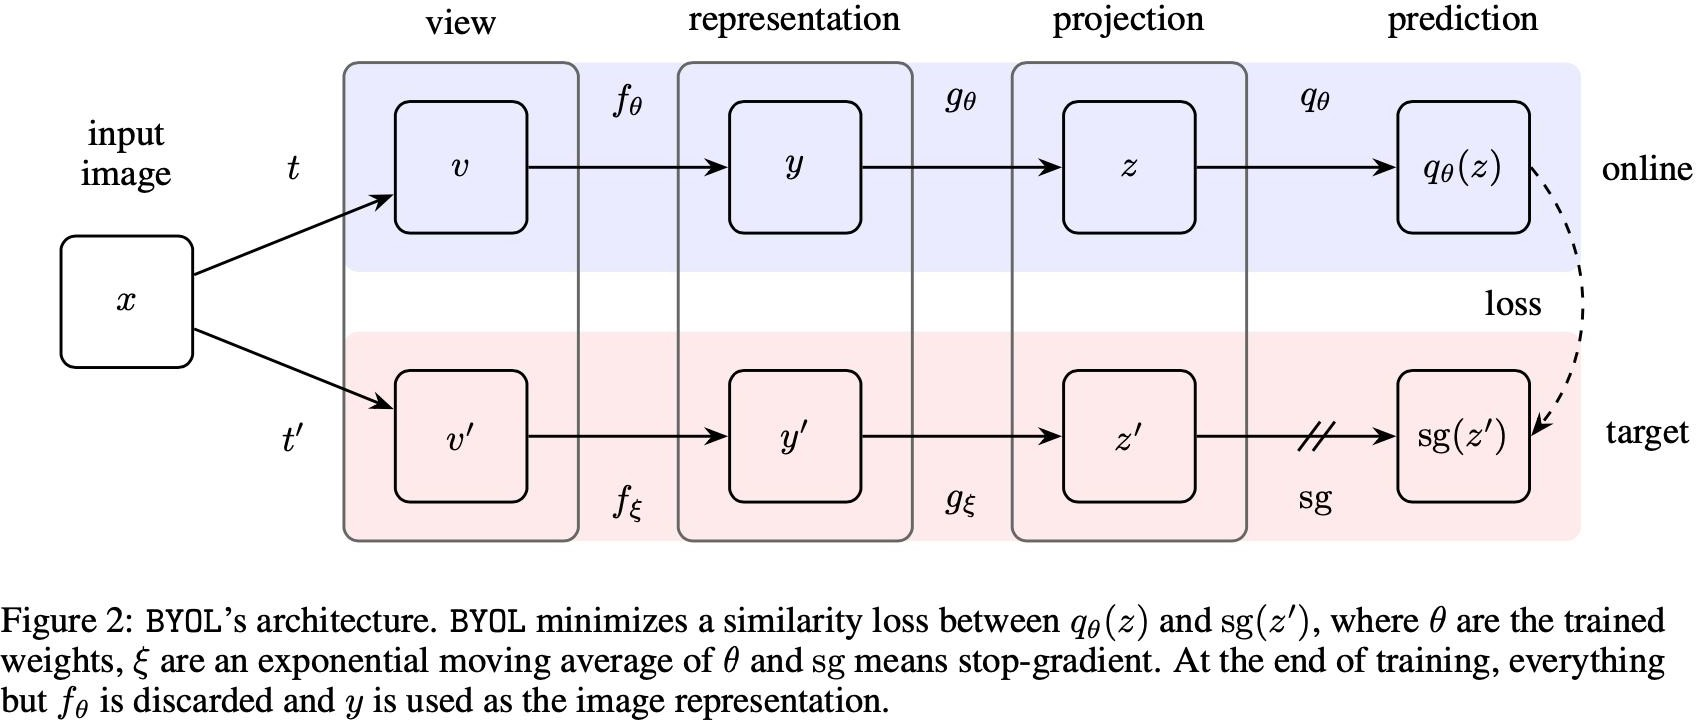
\includegraphics[width=\linewidth,height=0.9\textheight,keepaspectratio]{images/contrastive/slide_81_1_img.jpg}
\end{figure}

\framebreak

\textbf{How does BYOL work?}
\begin{itemize}
    \item There are two networks: an \textbf{online network} and a \textbf{target network}. Both start out the same.
    \item Each network has an encoder (think of it as a feature extractor).
    \item The online network has an extra part called the \textbf{predictor head}.
    \item The target network's parameters are updated slowly using the online network's parameters (using something called an exponential moving average).
    \item The goal is simple: make the online network's prediction as close as possible to the target network's output, using mean squared error between their normalized outputs.
\end{itemize}

\framebreak

\begin{figure}
    \centering
    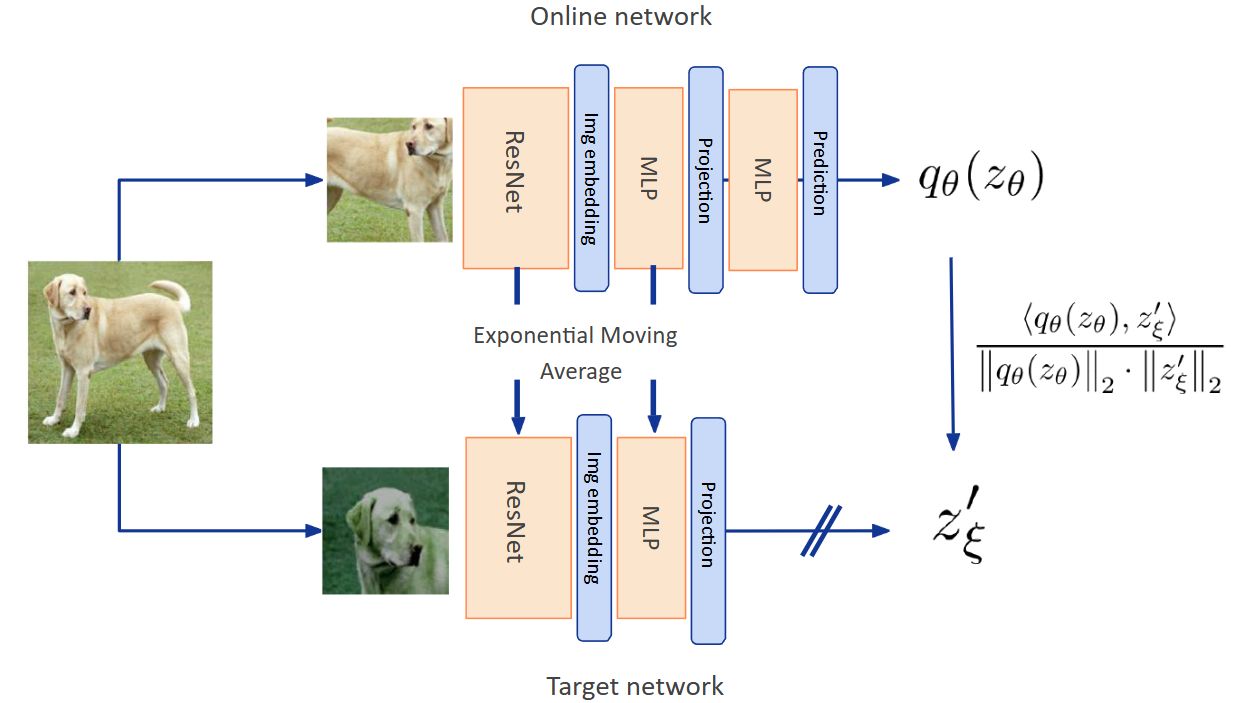
\includegraphics[width=\linewidth,height=0.9\textheight,keepaspectratio]{images/contrastive/slide_82_1_img.png}
\end{figure}

\framebreak

\begin{figure}
    \centering
    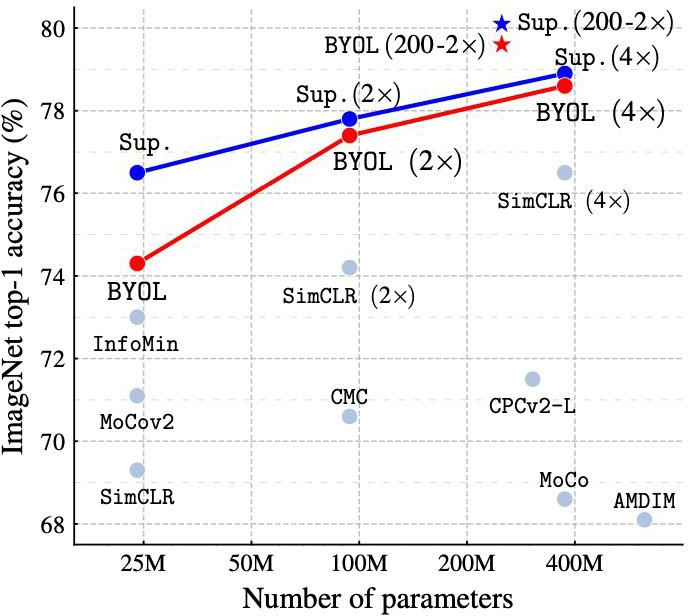
\includegraphics[width=\linewidth,height=0.9\textheight,keepaspectratio]{images/contrastive/slide_83_1_img.jpg}
\end{figure}

\framebreak

\begin{figure}
    \centering
    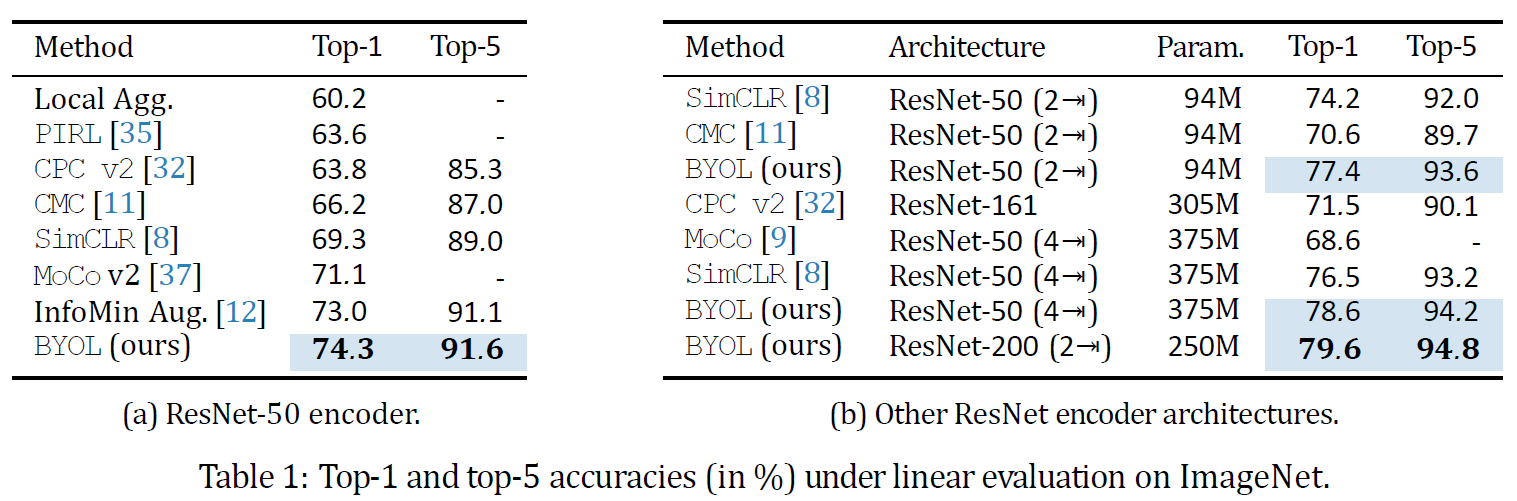
\includegraphics[width=\linewidth,height=0.9\textheight,keepaspectratio]{images/contrastive/slide_84_1_img.png}
\end{figure}

\framebreak

\begin{figure}
    \centering
    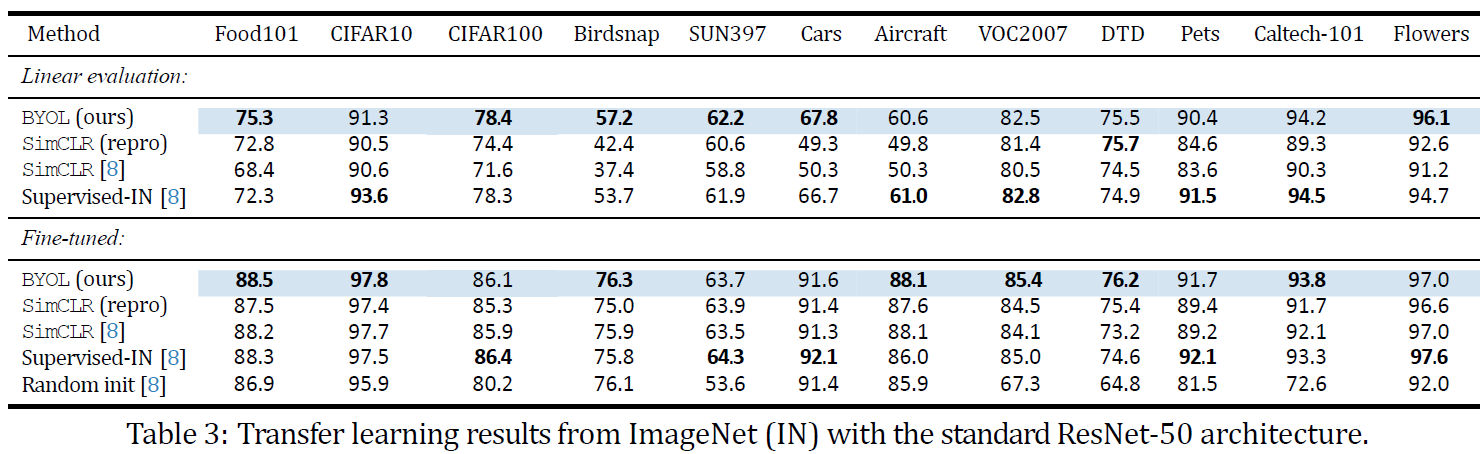
\includegraphics[width=\linewidth,height=0.9\textheight,keepaspectratio]{images/contrastive/slide_85_1_img.png}
\end{figure}

\framebreak

\textbf{What's special about BYOL?}
\begin{itemize}
    \item Even though there are no explicit negatives, the difference between the online and target networks acts like a source of "negative" information.
    \item This means we don't need huge batch sizes or to search for negative samples.
    \item BYOL makes self-supervised learning simpler and more efficient!
\end{itemize}
\end{frame}